\documentclass[aspectratio=169,xcolor={dvipsnames,table}]{beamer}
\usepackage[no-math,deluxe,expert,haranoaji]{luatexja-preset}
\usepackage{luatexja-otf}
\renewcommand{\kanjifamilydefault}{\gtdefault}
\renewcommand{\emph}[1]{{\upshape\bfseries #1}}
\usetheme{metropolis}
\metroset{block=fill}
\setbeamertemplate{navigation symbols}{}
\setbeamertemplate{blocks}[rounded][shadow=false]
\usecolortheme[rgb={0.7,0.2,0.2}]{structure}
%%%%%%%%%%%%%%%%%%%%%%%%%%%
\usepackage{media9}
\usepackage[absolute,overlay]{textpos}
%\usepackage[grid=true,gridcolor=Maroon,subgridcolor=gray,gridunit=pt,texcoord]{eso-pic} %場所決めのためのgrid表示
%%%%%%%%%%%%%%%%%%%%%%%%%%%
%% さまざまなアイコン
%%%%%%%%%%%%%%%%%%%%%%%%%%%
\usepackage{fontawesome}
%\usepackage{figchild}
\usepackage{twemojis}
\usepackage{utfsym}
\usepackage{bclogo}
\usepackage{marvosym}
\usepackage{fontmfizz}
\usepackage{pifont}
\usepackage{phaistos}
\usepackage{worldflags}
\usepackage{jigsaw}
%%%%%%%%%%%%%%%%%%%%%%%%%%%
\usepackage{tikz}
\usetikzlibrary{backgrounds}
\usepackage{tcolorbox}
\usepackage{tikzpeople}
\usepackage{tikzlings}
\usepackage{tikzducks}
\usepackage{circledsteps}
\usepackage{xcolor}
\usepackage{amsmath}
\usepackage{booktabs}
\usepackage{chronology}
\usepackage{signchart}
\usepackage{tipa}
\usepackage{pxrubrica}
%%%%%%%%%%%%%%%%%%%%%%%%%%%
%% 場合分け
\usepackage{cases}
%%%%%%%%%%%%%%%%%%%%%%%%%%%
% \myAnch{<名前>}{<色>}{<テキスト>}
% 指定のテキストを指定の色の四角枠で囲み, 指定の名前をもつTikZの
% ノードとして出力する. 図には remeber picture 属性を付けている
% ので外部から参照可能である.
\newcommand*{\myAnch}[3]{%
  \tikz[remember picture,baseline=(#1.base)]
    \node[draw,rectangle,#2] (#1) {\normalcolor #3};
}
%%%%%%%%%%%%%%%%%%%%%%%%%%%%
%% 音声リンク表示
\newcommand{\myaudio}[1]{\href{#1}{\faVolumeUp}}
%%%%%%%%%%%%%%%%%%%%%%%%%%%
% \myEmph コマンドの定義
%\newcommand{\myEmph}[3]{%
%    \textbf<#1>{\color<#1>{#2}{#3}}%
%}
\usepackage{xparse} % xparseパッケージの読み込み
\NewDocumentCommand{\myEmph}{O{} m m}{%
    \def\argOne{#1}%
    \ifx\argOne\empty
        \textbf{\color{#2}{#3}}% オプション引数が省略された場合
    \else
        \textbf<#1>{\color<#1>{#2}{#3}}% オプション引数が指定された場合
    \fi
}
%%%%%%%%%%%%%%%%%%%%%%%%%%%
%% 文末の上昇イントネーション記号 \myRisingPitch
%% 通常のイントネーション \myDownwardPitch
%% https://note.com/dan_oyama/n/n8be58e8797b2
%%%%%%%%%%%%%%%%%%%%%%%%%%%
\newcommand{\myRisingPitch}{
\begin{tikzpicture}[scale=0.3,baseline=0.3]
\draw[->,>=stealth] (0,0) to[bend right=45] (1,1);
\end{tikzpicture}
}
\newcommand{\myDownwardPitch}{
\begin{tikzpicture}[scale=0.3,baseline=0.3]
\draw[->,>=stealth] (0,1) to[bend left=45] (1,0);
\end{tikzpicture}
}
%%%%%%%%%%%%%%%%%%%%%%%%%%%
\title{English is fun.}
\subtitle{I have watched the movie three times.}
  \author{}
\institute[]{}
\date[]

%%%%%%%%%%%%%%%%%%%%%%%%%%%%
%% TEXT
%%%%%%%%%%%%%%%%%%%%%%%%%%%%
\begin{document}
\begin{frame}[plain]
  \titlepage
\end{frame}

\section*{授業の流れ}
\begin{frame}[plain]
  \frametitle{授業の流れ}
  \tableofcontents
\end{frame}

%%%%%%%%%%%%%%%%%%%%%%%%%%%%%%%%
%%%%%%%%%%%%%%%%%%%%%%%%
\section*{現在完了とは(復習)}
%%%%%%%%%%%%%%%%%%%%%%%%%%%%
\begin{frame}[plain]{現在完了とは(復習)}
 \begin{enumerate}
 \item Jane \textcolor{NavyBlue}{\bfseries has stayed} in London for six years.
 \item I \textcolor{NavyBlue}{\bfseries have watched} the movie three times.
 \item Bob \textcolor{NavyBlue}{\bfseries has lost} his bag.
\end{enumerate}

\vspace{30pt}

 \begin{block}<2->{現在完了の基本}
\small
\begin{itemize}\setbeamertemplate{items}[square]
 \item<3->  現在完了形\,\Circled[fill color=white]{\,\textbf{have} $+$ 過去分詞\,}\,は「過去と現在にまたがる表現」です\\
\hfill\visible<4->{{\scriptsize 主語が三人称単数のときは$\textcolor{NavyBlue}{\text{\bfseries has} + \text{過去分詞}}$}}
 \item \visible<5->{過去分詞は\kenten{受け身}とならんで\kenten{完了}の意味をあらわします}%
\end{itemize}
      \end{block}
\hfill{\tiny 0144}\,{\scriptsize \myaudio{./audio/013_have_pp_keiken_01.mp3}}

\begin{textblock*}{0.4\linewidth}(365pt,50pt)
\visible<1->{\begin{tikzpicture}
\duck[signpost=\scalebox{0.3}{
\parbox{2.5cm}{\color{black}\centering
{\Large 現在完了$=$\\過去$+$現在}}},
signcolour=brown!70!gray,
signback=white!80!brown,
graduate=gray!20!black,
tassel=red!70!black,
laughing,
%speech={\tiny 反復練習!}
]
\end{tikzpicture}}
\end{textblock*}
\end{frame}
%%%%%%%%%%%%%%%%%%%%%%%%
%%%%%%%%%%%%%%%%%%%%%%%%%%%%%%%%%%%%%%%%%%%
\section{経験をあらわす現在完了}
%%%%%%%%%%%%%%%%%%%%%%%%%%%%%%%%%%%%%%%%%%
\begin{frame}[plain]{現在完了--経験--}
 
\visible<1->{\begin{enumerate}%\setcounter{enumi}{1}
 \item $\left\{\begin{tabular}{rl}
(A)& I \textcolor{Maroon}{\bfseries visited} the tower two years ago.\hspace{9\zw}{\scriptsize tower \textipa{/t\'aU\textrhookschwa /} 塔、タワー}\\
(B)& I \textcolor{NavyBlue}{\bfseries have visited} the tower three times.
\end{tabular}
\right.$
\end{enumerate}}

\visible<2->{\signchart[width=10,height=.5]{,,,,{\textcolor{Maroon}{\textbf{visited}}},,,今}{,,},}
\visible<3->{\signchart[width=10,height=.5]{1回目,,2回目,,{\textcolor{NavyBlue}{\textbf{have visited}}},,3回目,今}{,,,}}

\begin{tikzpicture}[overlay]
%\draw[gray!50] (0,0) grid (12,5);
 %\fill[ForestGreen!70,opacity=.5] (11.57,3.75) circle [radius=.25];
\visible<2->{ \fill[Maroon!90,opacity=.75] (7.57,3.72) circle [radius=.25];}
\visible<3->{\fill[NavyBlue!90,opacity=.75] (3.1,1.21) circle [radius=.25];
\fill[NavyBlue!90,opacity=.75] (5.35,1.21) circle [radius=.25];
\fill[NavyBlue!90,opacity=.75] (9.78,1.21) circle [radius=.25];}
%\node[fill=NavyBlue!90,opacity=.75] at (10.88,1.21) { };
\visible<4->{\node[] at (10.89,1.21) {\LARGE \textcolor{NavyBlue}{x }};
\node[] at (10.9,.4) {\scriptsize \begin{tabular}{c}
				   これまでに\\
				 3回訪れた\\
				  ことがある\end{tabular}};}
% \draw[NavyBlue!70,line width=6pt,opacity=.7] (4.2,1.21) -- (10.9,1.21);
\end{tikzpicture}

\visible<5->{{\scriptsize 過去から現在までの\kenten{経験}を表しています}}%
\hfill{\tiny 0117}\,{\scriptsize \myaudio{./audio/013_have_pp_keiken_02.mp3}}

\end{frame}
%%%%%%%%%%%%%%%%%%%%%%%%%%%%%%%%%%%%%
\section{回数を表す表現}
%%%%%%%%%%%%%%%%%%%%%%%%%%%%%%%%%%%%
\begin{frame}[plain]{回数}


 \begin{enumerate}
  \item<1-> I have met the singer \textcolor{Maroon}{\bfseries once}.\hfill{\scriptsize meet---met---met}\\
\visible<2->{\small わたしはその歌手に一度あったことがある。}
  \item<3-> My mother has visited Taiwan \textcolor{Maroon}{\bfseries twice}.\hfill{\scriptsize  visit---visited---visited}\\
\visible<4->{\small 母は台湾を二度訪れたことがある。}
  \item<5-> He has seen the movie \textcolor{Maroon}{\bfseries three times}.\hfill{\scriptsize  see---saw---seen}\\
\visible<6->{\small 彼はその映画を三回見たことがある。}
  \item<7-> They have traveled to Paris \textcolor{Maroon}{\bfseries many times}.\hfill{\scriptsize  travel---traveled---traveled :旅行する}\\
\visible<8->{\small 彼らはパリに何度も旅行したことがある。}%
\end{enumerate}

\vspace{-20pt}

\hfill{\tiny 0210}\,{\scriptsize \myaudio{./audio/013_have_pp_keiken_03.mp3}}

\begin{block}<9->{「何回」という表現}
\small

{\rowcolors{2}{NavyBlue!50}{yellow!50}
\begin{tabular}{ll}
{\scriptsize 意味}&{\scriptsize 英語}\\
1回 &once \textipa{/w\'2ns/}\\
2回 &twice \textipa{/tw\'aIs/}\\
3回& three times\\
\end{tabular}}
{\rowcolors{2}{NavyBlue!50}{yellow!50}
\begin{tabular}{ll}
&\\
4回&four times\\
5回&five times \\
6回&six times \\
\end{tabular}}
{\rowcolors{2}{NavyBlue!50}{yellow!50}
\begin{tabular}{ll}
&\\
7回&seven times\\
8回&eight times \\
9回&nine times \\
\end{tabular}}
{\rowcolors{2}{NavyBlue!50}{yellow!50}
\begin{tabular}{ll}
\makebox[0pt][l]{{\scriptsize    文の最後におきます}}\\[5pt]
10回&ten times\\
\multicolumn{1}{c}{$\vdots$}&\multicolumn{1}{c}{$\vdots$} \\
何回も&many times \\
\end{tabular}}
      \end{block}
\end{frame}
%%%%%%%%%%%%%%%%%%%%%%%%%%%%%%%%%%%%%%%%%%
\begin{frame}[plain]{回数}
 
\begin{textblock*}{0.4\linewidth}(100pt,50pt)
\visible<1->{\begin{tikzpicture}
\bear[
scale=2,
%speech={\scriptsize 現在完了},
signpost=\scalebox{1}{
\parbox{2.5cm}{\color{black}
\centering onceとtwiceこの2つは特別}},
signcolour= brown!70!gray,
signback=white!80!brown
]
\end{tikzpicture}}
\end{textblock*}

\begin{textblock*}{0.4\linewidth}(280pt,120pt)
\visible<2->{\begin{tikzpicture}
\duck[
scale=1.732,
signpost=\scalebox{0.5}{
\parbox{2.5cm}{\color{black}\centering
{\Large その他は\\数字 times}}},
signcolour=brown!70!gray,
signback=white!80!brown,
graduate=gray!20!black,
tassel=red!70!black,
laughing,
%speech={\tiny 反復練習!}
]
\end{tikzpicture}}
\end{textblock*}
\end{frame}
%%%%%%%%%%%%%%%%%%%%%%%%%%%%%%%%%%%%%%%%%%%
\section{neverとever}
%%%%%%%%%%%%%%%%%%%%%%%%%%%%%%%%%%%%%%%%%%%
\begin{frame}[plain]{neverとever}
\large

 \begin{enumerate}
  \item \visible<1->{I have \textcolor{Maroon}{\bfseries never} eaten sushi.}\hfill{}\visible<2->{{\scriptsize eat---ate---eaten}}
  \item \visible<3->{Have you \textcolor{NavyBlue}{\bfseries ever} climbed a mountain?}\hfill{}\visible<4->{{\scriptsize climb---climbed---climbed 登る}}
 \end{enumerate}
\hfill{\tiny 0113}\,{\scriptsize \myaudio{./audio/013_have_pp_keiken_04.mp3}}

\vfill

\begin{block}<5->{Topics for Today}
\small
\begin{itemize}\setbeamertemplate{items}[square]\small
 \item \visible<6->{{\bfseries never}は「今までに一度もない」(\kenten{未経験})}\\
I {\bfseries have never} $+$ 過去分詞 \ldots\,\,\,\textbf{.}{{\footnotesize (今までに一度も〜したことがない)}}
 \item \visible<7->{{\bfseries ever}は疑問文で用いて「今までに」\hfill{\kenten{経験の有無}をたずねる}}\\
\visible<8->{\textbf{Have you ever} $+$ 過去分詞 \ldots\,\,\,?{{\footnotesize (今までに〜したことがありますか)}}}
\end{itemize}
\end{block}
\end{frame}
%%%%%%%%%%%%%%%%%%%%%%%%%%%%
\begin{frame}[plain]{Exercises}

{\small あたえられた日本語の意味になるよう(~~~~~~~~)内の語句を並べ替えましょう。なお、先頭の語は大文字ではじめてください}%
\hfill{\tiny 0140}\,{\scriptsize \myaudio{./audio/013_have_pp_keiken_05.mp3}}

\vspace{-10pt}
 \begin{enumerate}
  \item あなたは今までにギターを弾いたことがありますか?\scalebox{3}{\twemoji{guitar}}\\
( you / have / ever / played ) the guitar?\\
\visible<2->{Have you ever played the guitar?}
\vspace{-10pt}
  \item あなたは今までにメキシコ料理を食べたことがありますか?\hfill\raisebox{-5pt}{\scalebox{3}{\twemoji{1f32e}}}\,\scalebox{.4}{\worldflag{MX}}\,\scalebox{3}{\twemoji{desert}}\\
( you / have / eaten / ever ) Mexican food?\\
\visible<3->{Have you ever eaten Mexican food?}
  \item 私は一度もジグソーパズルを買ったことがありません。\\
( never / have / I / bought ) a jigsaw puzzle.\\
\visible<4->{I have never bought a jigsaw puzzle.}
%  \item 私は一度も山に登ったことがない。
%(  climbed / I / never /  have ) a mountain.\\
%\visible<5->{I have never climbed a mountain.}
 \end{enumerate}

\vspace{-65pt}

\mbox{}\hfill\scalebox{.5}{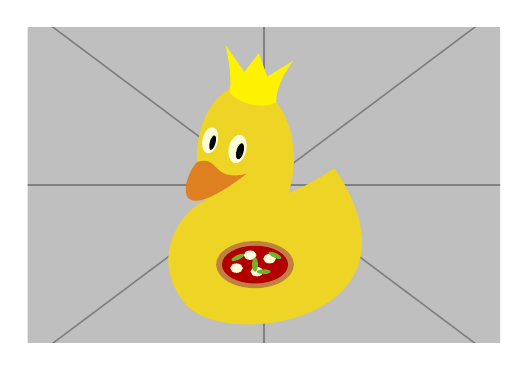
\begin{tikzpicture}
\clip (0,0) rectangle (6,4);
\node at (3,2) {%
\includegraphics[
width=8cm,height=6cm
]{example-image-duck}%
};
\jigsaw{6}{4}
\end{tikzpicture}}
\end{frame}
%%%%%%%%%%%%%%%%%%%%%%%%%%%%%%%%%%
%%%%%%%%%%%%%%%%%%%%%%%%%%%%%%%%%%%%%%%%%
\section{How many times  have you 〜?}
%%%%%%%%%%%%%%%%%%%%%%%%%%%%%%%%%%%%%%%%%
\begin{frame}[plain,t]{経験回数をたずねる}

\visible<1->{You have seen the movie \myAnch{long1}{Maroon}{three times}.}
 
\vspace{10pt}

\hfill\visible<2->{cf. \textcolor{NavyBlue}{\bfseries Have you seen} the movie three times?}

\vspace{10pt}

\visible<3->{\myAnch{long2}{Maroon}{\bfseries How many times} \textcolor{NavyBlue}{\bfseries have you seen} the movie?}%
%\hfill\visible<5->{{\small 何回?}}

\begin{tikzpicture}[remember picture,overlay]
 \visible<4->{\draw[Maroon,->,line width=3pt,opacity=.5.5] (long1.south) to[out=-90,in=90] node[sloped,above,text=black,font=\tiny,pos=.5]{How many timesに置き換え先頭へ} node[sloped,below,text=black,font=\tiny,pos=.5]{後ろは疑問文の語順} (long2.north);}
\end{tikzpicture}

\vspace{30pt}

\begin{block}<6->{Topics for Today}\small
\begin{itemize}\setbeamertemplate{items}[square]
 \item \visible<6->{$\textbf{\Circled[fill color=white]{\,How many times\,}\,\,have} + \textbf{S} + \text{過去分詞 \ldots ?}$}\hfill{「これまでに何回~したことがありますか」}
 \item \Circled[fill color=white]{\textbf{\,How many times\,}}\,\,の後ろは疑問文の語順

\end{itemize}
      \end{block}

\vspace{-10pt}

\hfill{\tiny 0142}\,{\scriptsize \myaudio{./audio/013_have_pp_keiken_06.mp3}}

\begin{textblock*}{0.4\linewidth}(300pt,90pt)
\visible<5->{\begin{tikzpicture}
\duck[signpost=\scalebox{0.22}{
\parbox{2.6cm}{\color{black}\centering
{\LARGE 今までの経験回数を聞く}}},
signcolour=brown!70!gray,
signback=white!80!brown,
graduate=gray!20!black,
tassel=red!70!black,
laughing,
speech={\tiny How many times?}
]
\end{tikzpicture}}
\end{textblock*}
\end{frame}
%%%%%%%%%%%%%%%%%%%%%%%%%%%%%%%%%
\section{まとめ}
%%%%%%%%%%%%%%%%%%%%%%%%%%%%%%%%
\begin{frame}[plain,t]{まとめ1}
 
\begin{block}<1->{\textcolor{black}{\mdseries 「経験」を表す現在完了}}
\small

\begin{itemize}\setbeamertemplate{items}[square]
 \item 「今までに~したことがある」のように\kenten{経験}を表すことがあります\\
\hfill{\scriptsize I {\bfseries have seen} the picture before.}
\end{itemize}
\end{block}

\begin{block}{\textcolor{black}{\mdseries never, ever}}
\small
\begin{itemize}\setbeamertemplate{items}[square]\small
 \item {\bfseries never}は「今までに一度もない」(\kenten{未経験})\\
I {\bfseries have never} $+$ 過去分詞 \ldots\,\,\,\textbf{.}{{\footnotesize (今までに一度も〜したことがない)}}\\

\hfill{\scriptsize I {\bfseries have never eaten} Mexican food.}
 \item {\bfseries ever}は疑問文で用いて「今までに」\hfill{\kenten{経験の有無}をたずねる}\\
{\bfseries Have} you  {\bfseries ever} $+$ 過去分詞 \ldots\,\,\,\textbf{?}{{\footnotesize (今までに〜したことがありますか)}}\\
\hfill{\scriptsize {\bfseries Have} you {\bfseries ever eaten} sushi?}
\end{itemize}
\end{block}
\end{frame}
%%%%%%%%%%%%%%%%%%%%%%%%%
\begin{frame}[plain,t]{まとめ2}
 \begin{block}{\textcolor{black}{\mdseries 経験回数をたずねる}}\small
\begin{itemize}\setbeamertemplate{items}[square]
 \item \Circled[fill color=white]{\,\textbf{How many times}\,}\,\,\textbf{have} $+$ \textbf{S} $+$ 過去分詞 \ldots ?\hfill{「これまでに何回~したことがありますか」}
 \item \Circled[fill color=white]{\,\textbf{How many times}\,}\,\,の後ろは疑問文の語順\\
\hfill{}{\scriptsize {\bfseries How many times} have you seen the movie?}

\end{itemize}
      \end{block}

\begin{block}{\textcolor{black}{\mdseries 「何回」という表現}}
\small

{\rowcolors{2}{NavyBlue!50}{yellow!50}
\begin{tabular}{ll}
{\scriptsize 意味}&{\scriptsize 英語}\\
1回 &once \\
2回 &twice \\
3回& three times\\
\end{tabular}}
{\rowcolors{2}{NavyBlue!50}{yellow!50}
\begin{tabular}{ll}
&\\
4回&four times\\
5回&five times \\
6回&six times \\
\end{tabular}}
{\rowcolors{2}{NavyBlue!50}{yellow!50}
\begin{tabular}{ll}
&\\
7回&seven times\\
8回&eight times \\
9回&nine times \\
\end{tabular}}
{\rowcolors{2}{NavyBlue!50}{yellow!50}
\begin{tabular}{ll}
\makebox[0pt][l]{{\scriptsize    文の最後におきます}}\\[5pt]
10回&ten times\\
\multicolumn{1}{c}{$\vdots$}&\multicolumn{1}{c}{$\vdots$} \\
何回も&many times \\
\end{tabular}}
      \end{block}

\hfill{\tiny 0303}\,{\scriptsize \myaudio{./audio/013_have_pp_keiken_07.mp3}}
\end{frame}
%%%%%%%%%%%%%%%%%%%%%%%%%%%%%
\end{document}
  \item  Have you ever eaten Mexican food?
